% Appendices A--E

\chapter{Sustainable Development Goals Achievement}
\label{app:sdg}

This appendix maps the project's objectives and outcomes to the United Nations Sustainable Development Goals (SDGs) referenced in Chapter~\ref{ch:intro}.

\textbf{SDG 9 --- Industry, Innovation, and Infrastructure.} The project contributes to resilient infrastructure and innovation in robotics by designing and implementing an autonomous UGV that can operate in disaster-affected environments where conventional communication and sensing are degraded. The multi-tier communication architecture (Wi-Fi, 4G, mesh, LoRa) and deployable mesh nodes provide resilient connectivity that can support not only the UGV but also follow-on missions and other robots. The integration of open-source and commodity components (ROS~2, Raspberry Pi~4, ESP32 DevKit, YDLidar, Kinect v1) demonstrates innovation within resource constraints and supports replicability and adaptation by other groups.

\textbf{SDG 11 --- Sustainable Cities and Communities.} The project aims to enhance the safety and sustainability of human settlements by improving the capability to assess disaster sites and support rescue operations without unnecessarily exposing responders to risk. The UGV delivers mapping, hazard detection, and natural-language reporting so that operators can make informed decisions about entry and resource allocation. By reducing the cognitive load on operators through AI-driven summarisation and spatial decision memory, the system supports more efficient and safer disaster response, aligning with the goal of making cities and communities more resilient and sustainable.

\chapter{Source Code and Repository Structure}
\label{app:code}

The project is software-heavy and uses ROS~2 (C++/Python), Python (FastAPI, YOLOv8, ProxMaP-style model), and JavaScript (web dashboard). No HDL or C-only codebase is applicable; the following describes the main software components and where source code or representative listings can be provided.

\textbf{Onboard stack (UGV).} ROS~2 packages include Cartographer for SLAM, Nav2 for navigation, and a custom frontier exploration package (frontier\_explorer) that implements frontier detection, BFS clustering, scoring with heading bonus, and integration with a ProxMaP-style map predictor node. The map predictor node runs a U-Net on 128$\times$128 robot-centred map crops and publishes a predicted map topic used by the frontier explorer. Configuration and launch files for sensors, TF, and Nav2 costmaps (including Kinect v1 in the local costmap) are part of the repository.

\textbf{Ground control station and AI.} The perception backend (Groq Brain) is a FastAPI application that exposes an endpoint for frame processing: it runs three YOLOv8 models, calls a Groq-hosted LLM (Llama-4-Scout) for scene and hazard analysis, and performs spatial decision memory (X-SDM) and person profiling. It publishes map annotations to a ROS~2 topic consumed by the dashboard. The dashboard is a JavaScript frontend that connects to the robot via rosbridge (WebSocket) and to the perception API, displaying camera streams, map, detections, teleop controls, and battery/network status.

\textbf{Repository.} Full source code is publicly available at \url{https://github.com/habeelali/fyp-indoor-ugv} \cite{fyprepo}. The repository includes the ROS~2 packages, the perception backend, the web dashboard, configuration files, and documentation.

\chapter{Hardware Schematics}
\label{app:schematics}

This appendix references the hardware architecture of the UGV and the communication infrastructure. Full schematic diagrams can be included or attached as separate sheets.

\textbf{Power distribution.} The UGV is powered by a 24\,V pack comprising two 3s3p 18650 cell groups in series. The high-power branch supplies unregulated 24\,V to the motor drivers; the low-power branch uses a buck converter to provide a regulated 5\,V rail for the Raspberry Pi~4, sensors (LiDAR, Kinect v1, USB webcam), ESP32-CAM, router (Archer C6), and headlights. The deployable mesh nodes are each powered by a 2500\,mAh LiPo. The LoRa SX1278 and ESP32 DevKit modules on the UGV are powered from the 5\,V rail or appropriate regulation.

\textbf{Connectivity.} The Raspberry Pi~4 connects to the YDLidar X3 via USB--UART, to the Kinect v1 via USB, and to the USB webcam via USB. The ESP32-CAM (rear) communicates over Wi-Fi or a dedicated link. The Pi is connected to the Archer C6 router via Ethernet. The servo for mesh node deployment and the ESP32 DevKit mesh modules are interfaced to the Pi or to the main power/control bus as per the physical design. The LoRa SX1278 is connected to an MCU (e.g.\ ESP32) or to the Pi via UART/SPI depending on the driver implementation.

% --- FIGURE PLACEHOLDER: Block diagram (power/connectivity) ---
% Add file: figures/hardware_block.pdf or .png
\begin{figure}[htbp]
\centering
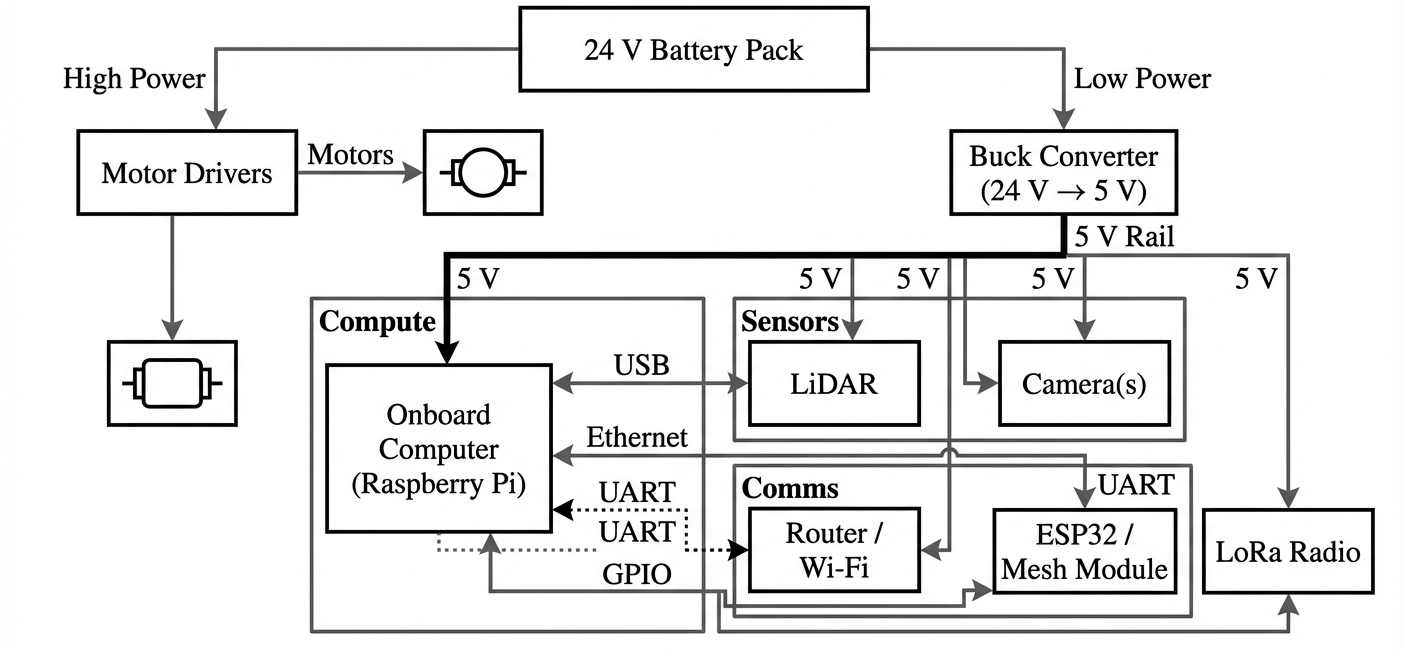
\includegraphics[width=0.9\textwidth]{figures/hardware_block.png}
\caption{UGV hardware block diagram (power and connectivity).}
\label{fig:hardwareblock}
\end{figure}

\chapter{List of Components}
\label{app:components}

The following table lists the main components of the as-built system with part or model identifiers and approximate acquisition costs in Pakistani Rupees (PKR), as recorded at procurement (indicative; market prices vary).

\begin{table}[htbp]
\caption{Bill of materials (BOM) with indicative costs (PKR).}
\label{tab:bom}
\centering
\small
\begin{tabular}{p{1.7cm}p{2.1cm}p{3.2cm}r}
\toprule
\textbf{Item} & \textbf{Part / model} & \textbf{Specification} & \textbf{PKR} \\
\midrule
Compute & RPi~4 Model B & 8\,GB RAM, Ubuntu 22.04, ROS~2 & 25\,000 \\
2D LiDAR & YDLidar X3 & 12\,m, 10\,Hz, USB--UART & 20\,000 \\
RGB-D & Kinect v1 & Point cloud, local costmap & 5\,000 \\
Main camera & USB webcam & 720p, 15\,fps & --- \\
Rear camera & ESP32-CAM & 720p, 15\,fps & 1\,800 \\
Wi-Fi (UGV) & Archer C6 & Dual-band, Ethernet, AP & 12\,000 \\
Wi-Fi (GCS) & Tenda F3 & Indoor / hotspot client & 4\,500 \\
Mesh node & ESP32 DevKit & ESP-WiFi-MESH; 2$\times$ @ 1\,000 & 2\,000 \\
Mesh battery & 2500\,mAh LiPo & Per deployable node; 2$\times$ @ 500 & 1\,000 \\
Deployment & Servo & Node drop along path & --- \\
LoRa & SX1278 (433\,MHz) & 2$\times$ modules (pair) & 5\,000 \\
UGV battery & 18650 (3s3p$\times$2) & 24\,V pack, BMS & 7\,500 \\
Converter & 24\,V--5\,V buck & 5\,V rail & 1\,500 \\
Chassis & 4WD skid-steer & Motors, wheels, drivers & 15\,000 \\
Lights & LED + strobe & Low-light & --- \\
\midrule
\multicolumn{3}{r}{\textbf{Subtotal (priced lines above)}} & \textbf{100\,300} \\
\midrule
\multicolumn{4}{p{10.8cm}}{\textit{Software (no unit hardware cost listed):} ROS~2 Humble, Cartographer, Nav2, frontier explorer \& map predictor, FastAPI, YOLOv8, Llama-4-Scout, web dashboard (rosbridge). GCS workstation GPU assumed available separately.} \\
\bottomrule
\end{tabular}
\end{table}

\chapter{Project Timeline}
\label{app:timeline}

The project ran from June 2025 to March 2026. The following timeline summarises the main phases.

\begin{itemize}
\item \textbf{Phase 1 --- Design and literature (June--August 2025):} Problem definition, objectives, literature review, and system architecture (conceptual framework, high-level design, subsystem design for power, locomotion, perception, SLAM, navigation, frontier exploration, communication, vision/AI, GCS). Corresponds to Chapters 1--3 of the thesis.

\item \textbf{Phase 2 --- Implementation Component 1 (September--October 2025):} Hardware procurement and assembly (chassis, Pi~4, YDLidar X3, Kinect v1, USB webcam, ESP32-CAM, Archer C6, mesh nodes with ESP32 DevKit and servo, LoRa SX1278, 24\,V battery). Software setup (Ubuntu 22.04, ROS~2 Humble, Cartographer, Nav2, custom frontier explorer and map predictor). Integration and basic validation of SLAM, navigation, and exploration.

\item \textbf{Phase 3 --- Implementation Component 2 (November--December 2025):} Communication stack (Wi-Fi, 4G, mesh deployment and routing table update, LoRa). GCS and AI pipeline (FastAPI backend, YOLOv8, Llama-4-Scout, X-SDM, person profiling, mission logs, ROS~2 annotations). Web dashboard (camera streams, map, detections, teleop, battery/network). Integration and end-to-end tests.

\item \textbf{Phase 4 --- Testing and evaluation (January 2026):} Unit testing (SLAM, Nav2, frontier explorer, map predictor, perception pipeline, mesh, LoRa). Function testing (Requirements A, B, C; scenarios 1--3). Evaluation in the 40$\times$30\,m test environment. Data collection for mapping, communication, detection, and frontier scoring (with vs.\ without prediction).

\item \textbf{Phase 5 --- Report and dissemination (February--March 2026):} Analysis of results, comparison with objectives and related work, socio-economic and environmental impact. Thesis writing (Ch 4--6), appendices, and bibliography. Conference paper preparation and submission. Final year project presentation and viva.
\end{itemize}
